\documentclass[a4paper,12pt]{article}
\usepackage[a4paper, total={180mm, 272mm}]{geometry}

\usepackage{fontspec}
\setmainfont[Path=fonts/, Extension=.ttf]{ipaexm}

\setlength\parindent{3.5em}
\setlength\parskip{0em}
\renewcommand{\baselinestretch}{1.247}

\usepackage{graphicx}
\graphicspath{{images/}}

\begin{document}

\thispagestyle{empty}

\Large
\noindent \\
Radial Blur Ino\medskip
\par
\normalsize
Generate an average value Blur in a radial direction.\par
It is also possible to add a twist to the direction (processing time will increase).\\
\par
First, it processes the Alpha channel if specified.\par
Then, it processes the RGB pixels where the Alpha channel is not zero.\par
When Alpha channel is not processed, it will mask the changes in the\par
RGB image using the Alpha values. Therefore, the original image edges will remain.\\
\\
-{-}- \ Inputs \ -{-}-\\
Source\par
Connect the image to be processed.\\
Reference\par
Connect the reference image to assign the strength of the effect into each pixel.\\
\\
\\
-{-}- \ Settings \ -{-}-\\
Center\par
Specify the center position from where to radiate.\par
Origin is the center of the image to be processed. Not the center of the camera.\par
The unit is millimeters.\par
The default value is the center of the image at \textquotedbl 0.0 0.0\textquotedbl .\\
\\
Radius\par
Specify a radius from the center that will not get blurred.\par
The unit is millimeters.\par
Value could be greater than or equal to 0.\par
The default value is 0, which will cause blur in the whole image.\\
\\
Blur\par
Allows to adjust the intensity of the blur.\par
The strength of the blur is determined by the distance from the Center to each pixel.\par
The calculation formula is: (Pixel\_Len - Radius) * (Blur / 100), where Pixel\_Len being\par 
the distance of each pixel from the center.\par
At the minimum value of 0, there will be no blur. The maximum value is 100.\par
The default value is 1.

\newpage

\thispagestyle{empty}

\ \vspace{-0.2em}
\par
\noindent Twist\par
Allows to add a twist.\par
Define how many turns there will be from the Center to the reference distance.\par
The reference distance is half the height of the resulting image.\par
At the minimum value of 0, there will be no twist. The maximum value is 180.\\
\\
Alpha Rendering\par
This option is valid only when there is an Alpha channel.\par
When inactive, it masks the changes in the RGB values using the original Alpha\par 
of the image.\par
When active, the effect will be able to modify the Alpha channel, extending it\par 
as necessary to reproduce the full span of the effect.\par
The default setting is active.\\
\\
Anti Alias\par
Allows to add an antialiasing process, in order to eliminate jagged edges.\par
The result will become smoother, but it will take more time to process.\par
The default setting is OFF.\par
<Processing time reference examples>\par
Width=2176 Height=1236 Center=0,0 Radius=0 Blur=3 Alpha=ON\par
Shrink=1\par
\noindent \hskip 7em Twist=0\par
\noindent \hskip 10.5em Anti Alias=OFF ~7sec\par
\noindent \hskip 10.5em Anti Alias=ON \, ~32sec\par
\noindent \hskip 7em Twist=1-180\par
\noindent \hskip 10.5em Anti Alias=OFF ~19sec\par
\noindent \hskip 10.5em Anti Alias=ON \, ~780sec\par
Shrink=3\par
\noindent \hskip 7em Twist=0\par
\noindent \hskip 10.5em Anti Alias=OFF ~3sec\par
\noindent \hskip 10.5em Anti Alias=ON \, ~4sec\par
\noindent \hskip 7em Twist=1-180\par
\noindent \hskip 10.5em Anti Alias=OFF ~4sec\par
\noindent \hskip 10.5em Anti Alias=ON \, ~34sec\\
\\
Reference\par
Choose how the Reference image values are used to set the strength of the effect\par 
into each pixel.\par
Choose from Red/Green/Blue/Alpha/Luminance.\par
Choose Nothing to disable the effect.\par
The default value is Red.

\newpage

\thispagestyle{empty}

\ \vspace{-0.2em}
\par
\noindent Radial Blur \ \ Reference Example

\large
\noindent \begin{picture}(0,0)
\put(170.5,-144.5){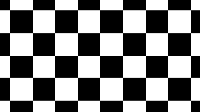
\includegraphics[width=13.3em]{RadialBlurInoOriginalImage}}
\put(92.5,-343){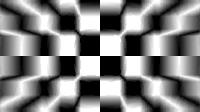
\includegraphics[width=13.3em]{RadialBlurInoRadialBlur30AAOFF}}
\put(314.5,-343){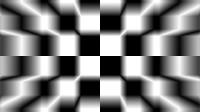
\includegraphics[width=13.3em]{RadialBlurInoRadialBlur30AAON}}
\put(92.5,-486){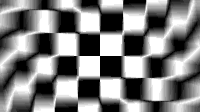
\includegraphics[width=13.3em]{RadialBlurInoTwistBlur20Twist45AAOFF}}
\put(314.5,-486){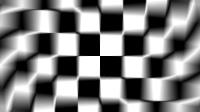
\includegraphics[width=13.3em]{RadialBlurInoTwistBlur20Twist45AAON}}
\put(26,-50){\normalsize{Original Image}}
\put(26,-67){\normalsize{(200x112pixel)}}
\put(89,-221){\normalsize{Anti Alias \ \ OFF}}
\put(311,-221){\normalsize{Anti Alias \ \ ON}}
\put(26,-249){\normalsize{Radial}}
\put(26,-267){\normalsize{(Blur 30)}}
\put(26,-382){\normalsize{Twist}}
\put(26,-400){\normalsize{(Blur 20}}
\put(32,-418){\normalsize{Twist 45)}}
\end{picture}\\[12.65em]

\end{document}